\documentclass[11pt,a4paper]{article}

\usepackage[utf8]{inputenc}
\usepackage[T1]{fontenc}
\usepackage{amsmath,amssymb,amsthm}
\usepackage{mathtools}
\usepackage{enumitem}
\usepackage{hyperref}
\usepackage{booktabs}
\usepackage{array}
\usepackage[margin=1in]{geometry}
\usepackage{listings}
\usepackage[x11names,table]{xcolor}
\usepackage{mdframed}
\usepackage{tikz}
\usetikzlibrary{positioning,arrows.meta,shapes.geometric,calc,decorations.pathreplacing}

% ---------- Code listing style for Lean ----------
\definecolor{codegreen}{rgb}{0,0.6,0}
\definecolor{codegray}{rgb}{0.5,0.5,0.5}
\definecolor{codepurple}{rgb}{0.58,0,0.82}
\definecolor{backcolour}{rgb}{0.95,0.95,0.92}

\lstdefinelanguage{Lean}{
  keywords={theorem, lemma, def, definition, axiom, structure, class, instance,
            by, exact, intro, intros, apply, refine, constructor, use, obtain,
            have, show, from, fun, assume, let, in, if, then, else,
            match, with, end, namespace, section, variable, variables,
            example, begin, sorry, admit, noncomputable, classical,
            import, open, export, private, protected, mutual, meta,
            do, for, while, return, try, catch, finally,
            Type, Prop, Sort, Type*, forall, exists, where, extends,
            set, push_neg, rw, simp, omega, nlinarith, linarith,
            ext, rfl, congr, fin_cases, haveI, letI, attribute},
  sensitive=true,
  morecomment=[l]{--},
  morecomment=[s]{/-}{-/},
  morestring=[b]",
  literate=
    {α}{{$\alpha$}}1 {β}{{$\beta$}}1 {γ}{{$\gamma$}}1
    {δ}{{$\delta$}}1 {ε}{{$\varepsilon$}}1 {ζ}{{$\zeta$}}1
    {η}{{$\eta$}}1 {θ}{{$\theta$}}1 {ι}{{$\iota$}}1
    {κ}{{$\kappa$}}1 {λ}{{$\lambda$}}1 {μ}{{$\mu$}}1
    {ν}{{$\nu$}}1 {ξ}{{$\xi$}}1 {π}{{$\pi$}}1
    {ρ}{{$\rho$}}1 {σ}{{$\sigma$}}1 {τ}{{$\tau$}}1
    {φ}{{$\varphi$}}1 {χ}{{$\chi$}}1 {ψ}{{$\psi$}}1
    {ω}{{$\omega$}}1 {Γ}{{$\Gamma$}}1 {Δ}{{$\Delta$}}1
    {Θ}{{$\Theta$}}1 {Λ}{{$\Lambda$}}1 {Σ}{{$\Sigma$}}1
    {Φ}{{$\Phi$}}1 {Ψ}{{$\Psi$}}1 {Ω}{{$\Omega$}}1
    {→}{{$\rightarrow$}}1 {←}{{$\leftarrow$}}1 {↔}{{$\leftrightarrow$}}1
    {⇒}{{$\Rightarrow$}}1 {⇐}{{$\Leftarrow$}}1 {⇔}{{$\Leftrightarrow$}}1
    {∀}{{$\forall$}}1 {∃}{{$\exists$}}1 {∈}{{$\in$}}1
    {∉}{{$\notin$}}1 {⊆}{{$\subseteq$}}1 {⊂}{{$\subset$}}1
    {∪}{{$\cup$}}1 {∩}{{$\cap$}}1 {≤}{{$\leq$}}1
    {≥}{{$\geq$}}1 {≠}{{$\neq$}}1 {≈}{{$\approx$}}1 {≃}{{$\simeq$}}1
    {≡}{{$\equiv$}}1 {∧}{{$\land$}}1 {∨}{{$\lor$}}1
    {¬}{{$\neg$}}1 {ℕ}{{$\mathbb{N}$}}1 {ℝ}{{$\mathbb{R}$}}1
    {ℂ}{{$\mathbb{C}$}}1 {ℤ}{{$\mathbb{Z}$}}1 {ℓ}{{$\ell$}}1
    {·}{{$\cdot$}}1 {∑}{{$\sum$}}1 {∏}{{$\prod$}}1
    {∅}{{$\emptyset$}}1 {∞}{{$\infty$}}1 {∂}{{$\partial$}}1
    {⟨}{{$\langle$}}1 {⟩}{{$\rangle$}}1 {…}{{$\ldots$}}1
    {₀}{{$_0$}}1 {₁}{{$_1$}}1 {₂}{{$_2$}}1 {⧸}{{$/$}}1 {‖}{{$\|$}}1
    {•}{{$\cdot$}}1 {⁻¹}{{$^{-1}$}}1 {⋆}{{$\star$}}1
    {∘}{{$\circ$}}1
    {⊓}{{$\sqcap$}}1 {⊥}{{$\bot$}}1 {⊤}{{$\top$}}1
    {ₗ}{{$_l$}}1 {ₘ}{{$_m$}}1 {ₙ}{{$_n$}}1
}

\lstdefinestyle{leanstyle}{
    language=Lean,
    backgroundcolor=\color{backcolour},
    commentstyle=\color{codegreen},
    keywordstyle=\color{blue},
    stringstyle=\color{codepurple},
    basicstyle=\ttfamily\footnotesize,
    breakatwhitespace=false,
    breaklines=true,
    captionpos=b,
    keepspaces=true,
    numbers=left,
    numbersep=5pt,
    showspaces=false,
    showstringspaces=false,
    showtabs=false,
    tabsize=2,
    numberstyle=\tiny\color{codegray}
}

\lstset{style=leanstyle}

\theoremstyle{plain}
\newtheorem{theorem}{Theorem}[section]
\newtheorem{proposition}[theorem]{Proposition}
\newtheorem{lemma}[theorem]{Lemma}
\newtheorem{corollary}[theorem]{Corollary}

\theoremstyle{definition}
\newtheorem{definition}[theorem]{Definition}
\newtheorem{example}[theorem]{Example}
\newtheorem{observation}[theorem]{Observation}

\theoremstyle{remark}
\newtheorem{remark}[theorem]{Remark}

\newcommand{\BISH}{\mathrm{BISH}}
\newcommand{\LPO}{\mathrm{LPO}}
\newcommand{\MP}{\mathrm{MP}}
\newcommand{\LLPO}{\mathrm{LLPO}}
\newcommand{\CLASS}{\mathrm{CLASS}}
\newcommand{\Hom}{\mathrm{Hom}}
\newcommand{\End}{\mathrm{End}}
\newcommand{\Gal}{\mathrm{Gal}}
\newcommand{\Frob}{\mathrm{Frob}}
\newcommand{\CH}{\mathrm{CH}}
\newcommand{\NS}{\mathrm{NS}}
\newcommand{\Lef}{\mathrm{Lef}}
\newcommand{\im}{\mathrm{im}}
\newcommand{\Spec}{\mathrm{Spec}}
\newcommand{\num}{\mathrm{num}}
\renewcommand{\hom}{\mathrm{hom}}
\newcommand{\prim}{\mathrm{prim}}
\newcommand{\Z}{\mathbb{Z}}
\newcommand{\Q}{\mathbb{Q}}
\newcommand{\R}{\mathbb{R}}
\newcommand{\C}{\mathbb{C}}
\newcommand{\F}{\mathbb{F}}
\newcommand{\Ql}{\Q_\ell}

\newcommand{\leanRepo}{\url{https://doi.org/10.5281/zenodo.18732559}}

\title{Decidability Transfer via Specialization:\\
Standard Conjecture~D for Abelian Threefolds\\[6pt]
\large (Paper~52, Constructive Reverse Mathematics Series)}

\author{Paul Chun-Kit Lee\thanks{Lean 4 formalization available at \leanRepo.}\\
\small Brooklyn, NY\\
\small \texttt{dr.paul.c.lee@gmail.com}}

\date{February 2026}

\begin{document}
\maketitle

\begin{abstract}
We prove that Standard Conjecture~D (numerical equivalence implies homological equivalence) for abelian varieties $A/\Q$ of dimension $g \le 3$ follows from the Tate conjecture for divisors---which is unconditional by Tate~(1966)---and the structural properties of the Lefschetz ring over finite fields, without invoking Standard Conjecture~B or characteristic~$0$ Hodge theory.

The proof transfers decidability from characteristic~$p$ to characteristic~$0$ via specialization.  The mechanism has three components: (i)~the smooth proper base change isomorphism identifies homological triviality across characteristics; (ii)~the Lefschetz ring of $A_p$ has unconditionally definite primitive components (Milne~2002, via the Rosati involution); (iii)~the liftable subspace $U = \im(\mathrm{sp})$ is stable under the Lefschetz operators $L$ and $\Lambda$ because the Fourier-Mukai transform specializes via the Poincar\'e bundle on the N\'eron model (K\"unnemann~1993, 1994).  For $g \le 3$, all Tate classes are Lefschetz classes---trivially for $g \le 2$ by dimensional constraints, and for $g = 3$ by the Hard Lefschetz isomorphism $L\colon H^2 \xrightarrow{\sim} H^4$ (Deligne, Weil~II) composed with Tate's theorem for divisors.  Non-degeneracy of~$U$ follows, yielding the transfer.

The argument fails sharply at dimension~$4$, where exotic Tate classes first appear outside the Lefschetz ring (Milne~2001, Example~1.8).  For even $g \ge 6$, Agugliaro~(2025) constructs non-Lefschetz Tate classes that are additionally non-liftable to characteristic~$0$.  This dimension-$4$ boundary matches the failure of the CM decidability rescue in Paper~50, providing independent confirmation that the Decidable Polarized Tannakian framework detects genuine arithmetic structure.

In the Constructive Reverse Mathematics interpretation, the result demonstrates that $\BISH$-decidable equality on numerical motives over $\F_p$ transfers to $\BISH$-decidable equality over $\Q$ through the algebraic shadow of the Archimedean polarization---the Lefschetz operators that survive reduction to characteristic~$p$.

The logical transfer architecture is formalized in Lean~4 over Mathlib; the bundle compiles with 0~errors, 0~warnings, and 0~\texttt{sorry}s, using zero custom axioms.
\end{abstract}

\medskip
\noindent\textbf{Disclaimer.} This proof is AI-assisted (Claude, Opus~4.6), and the author is a physician, not a domain expert in algebraic geometry. The results should be treated as preliminary until verified by specialists in the field.

\tableofcontents


%% ===================================================================
\section{Introduction}
\label{sec:intro}
%% ===================================================================

\subsection{Context}

Paper~50 of this series~\cite{Paper50} characterized Grothendieck's category of numerical motives by three logical axioms---decidable equality on morphism spaces (Standard Conjecture~D), algebraic spectrum, and Archimedean polarization---and posed five open questions.  The most consequential was Open Question~5:

\medskip
\noindent
\emph{Can the known decidability of numerical equivalence over $\F_p$ be transferred to $\Q$ via the specialization map on Chow groups?}
\medskip

This paper answers affirmatively for abelian varieties of dimension $g \le 3$.  It is part of a tetralogy (Papers~50--53): Paper~50 proposes the DPT axioms; Paper~51~\cite{Paper51} applies Axiom~3 to the rank-1 BSD conjecture; the present paper addresses the characteristic-crossing transfer; Paper~53~\cite{Paper53} provides a verified CM oracle and extends the computation to the dimension-$4$ boundary.

The progression from Paper~51 to the present paper is as follows.  Paper~51 showed that the positive-definite Archimedean metric (DPT Axiom~3) is the structural ingredient that rescues the rank-1 BSD generator search from MP to BISH: the N\'eron--Tate height's positive-definiteness over~$\R$ bounds the search space, while the $p$-adic analogue fails because $u(\Q_p) = 4$.  The natural next question is: does this Archimedean structure leave an \emph{algebraic shadow}---detectable purely in characteristic~$p$---capable of transferring decidability across the characteristic boundary?  The Lefschetz operators, which encode the algebraic skeleton of the Archimedean polarization and survive reduction mod~$p$ via the Rosati involution, are precisely this shadow.  The present paper proves the transfer works for $g \le 3$ and fails sharply at $g = 4$.

\subsection{The specialization strategy}

Let $A/\Z[1/N]$ be an abelian scheme with generic fiber $A_\Q$ and special fiber $A_p$ at a prime $p \nmid N$ of good reduction.  Fulton's specialization map on Chow groups,
\[
\mathrm{sp}\colon \CH^r(A_\Q) \longrightarrow \CH^r(A_p),
\]
is compatible with the cycle class map via the smooth proper base change isomorphism (SGA~$4\tfrac{1}{2}$; Fulton~\cite{Fulton}, Example~20.3.5).  The strategy is to use the known validity of Standard Conjecture~D over $\F_p$ (for classes where the Tate conjecture applies) to deduce it over~$\Q$.

The naive version of this strategy fails: the specialization map is not surjective on Chow groups.  New algebraic cycles appear in characteristic~$p$ (from extra endomorphisms), and a cycle that is numerically trivial over~$\Q$ might pair nontrivially with these non-liftable classes.  Bridging this gap requires proving that the liftable subspace $U = \im(\mathrm{sp})$ is non-degenerate with respect to the intersection pairing---and the only previously known proof of this non-degeneracy invokes Lieberman's Standard Conjecture~B over~$\Q$, which already implies Conjecture~D, creating a circularity.

We break the circularity for $g \le 3$ by showing that in these dimensions, all Tate classes are Lefschetz classes, so the unconditional definiteness of the Lefschetz ring (Milne~\cite{Milne2002}) suffices.


\subsection{Main results}

\begin{theorem}[Decidability transfer for $g \le 3$]
\label{thm:main}
Let $A/\Q$ be an abelian variety of dimension $g \le 3$.  Then Standard Conjecture~D holds for~$A$: if a cycle $Z \in \CH^r(A_\Q)$ is numerically trivial, then $Z$ is homologically trivial.

The proof uses only:
\begin{enumerate}[label=\emph{(\roman*)}]
\item the Tate conjecture for divisors on abelian varieties over $\F_p$ (unconditional; Tate~\cite{Tate1966});
\item the unconditional definiteness of the Lefschetz ring (Milne~\cite{Milne2002}, Remark~3.7);
\item the sub-Lefschetz stability of the liftable subspace (K\"unnemann~\cite{Kunnemann1993, Kunnemann1994});
\item the Hard Lefschetz theorem over $\F_p$ (Deligne~\cite{DeligneWeilII}).
\end{enumerate}
No appeal is made to Standard Conjecture~B, Hodge theory, or any characteristic~$0$ transcendental method.
\end{theorem}

\begin{theorem}[Sharp boundary at $g = 4$]
\label{thm:boundary}
The argument of Theorem~\ref{thm:main} fails at $g = 4$.  Exotic Tate classes in $H^4(A_p, \Ql(2))$---not generated by divisor classes---first appear for abelian fourfolds (Milne~\cite{Milne2001}, Example~1.8), as the characteristic~$p$ specializations of Anderson's exotic Weil classes.  For even $g \ge 6$, Agugliaro~\cite{Agugliaro2025} constructs non-Lefschetz Tate classes that are additionally non-liftable to Hodge classes of any CM-lifting.

This boundary coincides with the dimension-$4$ failure of the CM decidability rescue in Paper~50, Theorem~C, where Anderson's exotic Weil classes block the Hodge conjecture for CM abelian varieties.
\end{theorem}

\begin{observation}[CRM interpretation]
\label{obs:crm}
In the Constructive Reverse Mathematics framework, the result demonstrates decidability transfer across the characteristic boundary.  Over $\F_p$, the equality checker $Z \stackrel{?}{=}_\num 0$ is $\BISH$-decidable (the intersection pairing takes values in $\Z$, and Conjecture~D is known for abelian varieties in the Lefschetz range).  Over $\Q$, deciding whether $Z \equiv_\hom 0$ requires $\LPO$ for $\ell$-adic zero-testing.  The specialization map bridges the gap: the Lefschetz structure---the algebraic residue of the Archimedean polarization that survives reduction to characteristic~$p$---carries the $\BISH$-decidable verdict from $\F_p$ back to~$\Q$.
\end{observation}


% --- Figure 1: Specialization Transfer Architecture ---
\begin{figure}[ht]
\centering
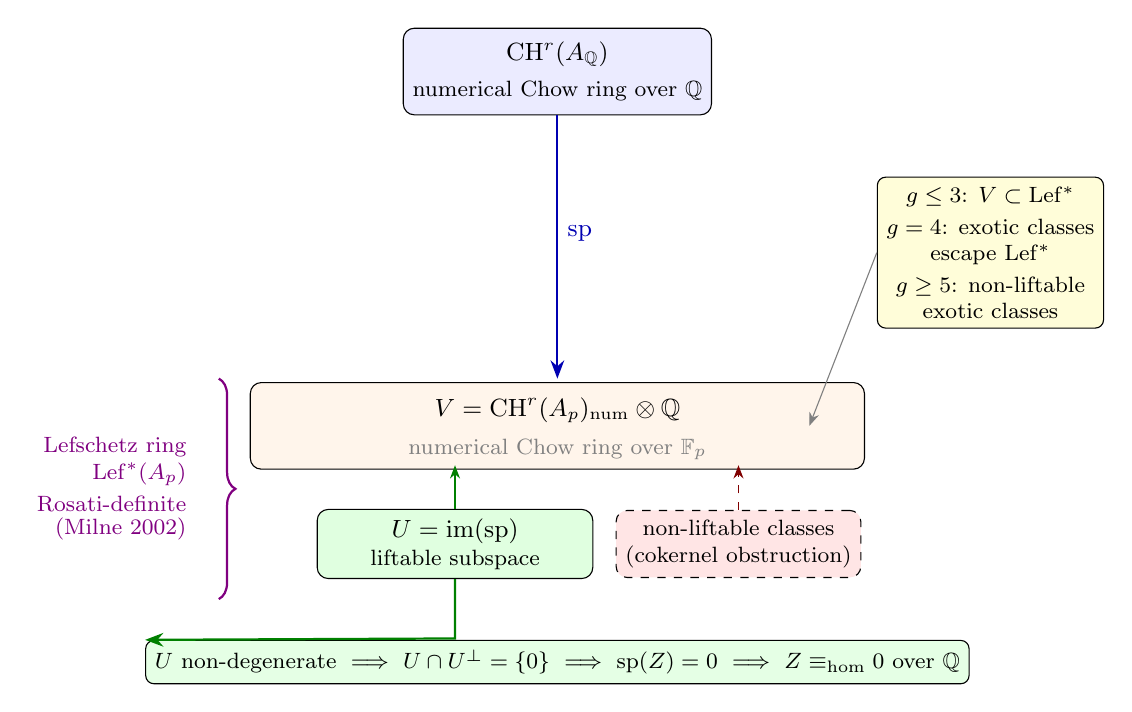
\begin{tikzpicture}[
  >=Stealth,
  box/.style={draw, rounded corners=4pt, minimum width=3.8cm, minimum height=1.1cm,
              align=center, font=\small},
  every node/.style={font=\small}
]

% --- Top: characteristic 0 ---
\node[box, fill=blue!8] (AQ) at (0,4.5) {$\CH^r(A_\Q)$\\[2pt]\footnotesize numerical Chow ring over $\Q$};

% --- Bottom: characteristic p ---
\node[box, fill=orange!8, minimum width=7.8cm] (V) at (0,0)
  {\phantom{$\CH^r(A_p)_\num \otimes \Q$}};
\node[font=\small] at (0,0.2) {$V = \CH^r(A_p)_\num \otimes \Q$};
\node[font=\footnotesize, text=gray] at (0,-0.3) {numerical Chow ring over $\F_p$};

% --- Liftable subspace inside V ---
\node[box, fill=green!12, minimum width=3.5cm, minimum height=0.7cm]
  (U) at (-1.3,-1.5) {$U = \im(\mathrm{sp})$\\[-1pt]\footnotesize liftable subspace};

% --- Non-liftable part ---
\node[box, fill=red!10, minimum width=3.0cm, minimum height=0.7cm, dashed]
  (coker) at (2.3,-1.5) {\footnotesize non-liftable classes\\[-1pt]\footnotesize (cokernel obstruction)};

% --- Specialization arrow ---
\draw[->, thick, blue!70!black] (AQ.south) -- node[right, pos=0.45] {$\mathrm{sp}$} (0,0.6);

% --- Containment arrows ---
\draw[->, thin, green!50!black] (U.north) -- (-1.3,-0.5);
\draw[->, thin, red!50!black, dashed] (coker.north) -- (2.3,-0.5);

% --- Lefschetz ring brace (left side) ---
\draw[decorate, decoration={brace, amplitude=6pt, mirror}, thick, violet]
  (-4.3,-2.2) -- (-4.3,0.6)
  node[midway, left=8pt, align=right, font=\footnotesize, text=violet]
  {Lefschetz ring\\$\Lef^*(A_p)$\\[2pt]\footnotesize Rosati-definite\\[-1pt]\footnotesize (Milne 2002)};

% --- Dimension annotation (right side) ---
\node[draw, rounded corners=3pt, fill=yellow!15, font=\footnotesize, align=center]
  (dim) at (5.5,2.2)
  {$g \le 3$: $V \subset \Lef^*$\\[2pt]
   $g = 4$: exotic classes\\escape $\Lef^*$\\[2pt]
   $g \ge 5$: non-liftable\\exotic classes};

\draw[->, thin, gray] (dim.west) -- (3.2,0);

% --- Key conclusion ---
\node[draw, rounded corners=3pt, fill=green!10, font=\footnotesize, align=center]
  (concl) at (0,-3.0)
  {$U$ non-degenerate $\;\Longrightarrow\;$ $U \cap U^\perp = \{0\}$
   $\;\Longrightarrow\;$ $\mathrm{sp}(Z) = 0$
   $\;\Longrightarrow\;$ $Z \equiv_\hom 0$ over $\Q$};

\draw[->, thick, green!50!black] (U.south) -- (-1.3,-2.7) -- (concl.north west);

\end{tikzpicture}
\caption{The specialization transfer architecture.  The specialization map $\mathrm{sp}$ sends cycles from characteristic~$0$ into the liftable subspace $U \subset V$.  For $g \le 3$, all algebraic classes on $A_p$ lie in the Lefschetz ring, where Rosati positivity guarantees definiteness.  The liftable subspace inherits this definiteness, forcing $U \cap U^\perp = \{0\}$ and completing the transfer.  At $g = 4$, exotic classes escape the Lefschetz ring, breaking the argument.}
\label{fig:transfer}
\end{figure}


%% ===================================================================
\section{Preliminaries}
\label{sec:prelim}
%% ===================================================================

We collect the key definitions and logical principles used throughout the paper.  No proofs appear in this section; the reader may consult Fulton~\cite{Fulton} for intersection theory, Milne~\cite{Milne2002} for the Lefschetz ring, and Bridges--Richman~\cite{BridgesRichman} for constructive foundations.

\begin{definition}[Standard Conjecture~D]
\label{def:conjD}
Let $A$ be a smooth projective variety over a field~$k$.  \emph{Standard Conjecture~D} asserts that numerical equivalence and homological equivalence coincide on algebraic cycles: if $Z \in \CH^r(A)$ satisfies $\deg(Z \cdot W) = 0$ for all $W \in \CH^{g-r}(A)$, then the cycle class $\mathrm{cl}(Z) = 0$ in $\ell$-adic cohomology.
\end{definition}

\begin{definition}[Specialization map]
\label{def:sp}
Given an abelian scheme $\mathcal{A}/\Z[1/N]$ with generic fiber $A_\Q$ and special fiber $A_p$ at a good prime $p$, the \emph{specialization map} $\mathrm{sp}\colon \CH^r(A_\Q) \to \CH^r(A_p)$ is defined via the Gysin homomorphism on the regular model.  It satisfies the compatibility $\mathrm{cl}_p \circ \mathrm{sp} = \mathrm{sp}_{\mathrm{coh}} \circ \mathrm{cl}_\Q$ with the cycle class maps (see Section~\ref{sec:naive} for the full diagram).
\end{definition}

\begin{definition}[Lefschetz ring]
\label{def:lefring_prelim}
For an abelian variety $A$ over a field $k$, the \emph{Lefschetz ring} $\Lef^*(A) \subset \CH^*(A)_\num \otimes \Q$ is the $\Q$-subalgebra generated by divisor classes under the intersection product.  Its definiteness properties are developed in Section~\ref{sec:lefschetz}.
\end{definition}

\begin{definition}[Logical principles]
\label{def:logic}
The proof operates within the following constructive hierarchy (see Bridges--Richman~\cite{BridgesRichman} for full definitions):
\begin{itemize}[nosep]
\item $\BISH$: Bishop's constructive mathematics---no omniscience principles.
\item $\LPO$ (Limited Principle of Omniscience): For any binary sequence $(a_n)$, either $\exists n\, (a_n = 1)$ or $\forall n\, (a_n = 0)$.  Required for zero-testing in $\Ql$.
\end{itemize}
The intersection pairing over $\F_p$ takes values in $\Z$, where equality is decidable in $\BISH$.  Over $\Q$, testing whether $\mathrm{cl}_\Q(Z) = 0$ in $H^{2r}(A_{\bar\Q}, \Ql(r))$ requires $\LPO$.
\end{definition}

\begin{remark}[Formalization scope]
\label{rem:scope_preview}
The Lean~4 formalization (Section~\ref{sec:formal}) covers the logical transfer architecture: the deduction from three geometric hypotheses (Propositions~\ref{prop:hom_transfer}, \ref{prop:num_partial}, and the Lefschetz decomposition of Sections~\ref{sec:lefschetz}--\ref{sec:dimension}) through a verified non-degeneracy lemma to Conjecture~D.  The deep geometric content of Sections~\ref{sec:lefschetz}--\ref{sec:dimension} enters the formalization as explicit hypotheses, not as axioms or sorries.
\end{remark}


%% ===================================================================
\section{The naive transfer and the cokernel obstruction}
\label{sec:naive}
%% ===================================================================

\subsection{Setup}

Let $A/\Z[1/N]$ be an abelian scheme of relative dimension~$g$, with generic fiber $A_\Q$ and special fiber $A_p$ at a prime $p \nmid N$.  Choose $\ell \ne p$.  The smooth proper base change theorem (SGA~$4\tfrac{1}{2}$) provides a canonical isomorphism
\[
\mathrm{sp}_{\mathrm{coh}}\colon H^{2r}_{\text{\'et}}(A_{\bar\Q}, \Ql(r)) \xrightarrow{\;\sim\;} H^{2r}_{\text{\'et}}(A_{\bar\F_p}, \Ql(r)).
\]
Fulton's specialization map on Chow groups, $\mathrm{sp}\colon \CH^r(A_\Q) \to \CH^r(A_p)$, defined via the Gysin homomorphism on the regular model, satisfies the compatibility
\begin{equation}
\label{eq:compat}
\mathrm{cl}_p \circ \mathrm{sp} = \mathrm{sp}_{\mathrm{coh}} \circ \mathrm{cl}_\Q
\end{equation}
where $\mathrm{cl}_\Q$ and $\mathrm{cl}_p$ are the cycle class maps over $\Q$ and $\F_p$ respectively.

\subsection{What transfers and what does not}

\begin{proposition}[Homological triviality transfers]
\label{prop:hom_transfer}
Let $Z \in \CH^r(A_\Q)$.  Then $\mathrm{cl}_\Q(Z) = 0$ if and only if $\mathrm{cl}_p(\mathrm{sp}(Z)) = 0$.
\end{proposition}

\begin{proof}
Immediate from~\eqref{eq:compat} and the fact that $\mathrm{sp}_{\mathrm{coh}}$ is an isomorphism.
\end{proof}

\noindent\emph{Lean role.}  This proposition enters the formalization as the hypothesis \texttt{Prop21~G}\,: if $\texttt{G.sp}\;Z = 0$ then $\texttt{G.is\_hom\_triv}\;Z$.  It is invoked at Step~7 of the main proof (see Table~\ref{tab:step_map}).

\begin{proposition}[Numerical triviality partially transfers]
\label{prop:num_partial}
Let $Z \in \CH^r(A_\Q)$ be numerically trivial over~$\Q$.  Then $\mathrm{sp}(Z)$ is orthogonal to $\im(\mathrm{sp}) \subset \CH^{g-r}(A_p)_\num$ with respect to the intersection pairing.
\end{proposition}

\begin{proof}
For any $W \in \CH^{g-r}(A_\Q)$, we have $\deg(\mathrm{sp}(Z) \cdot \mathrm{sp}(W))_{A_p} = \deg(Z \cdot W)_{A_\Q} = 0$ because specialization commutes with intersection products and the degree map.
\end{proof}

\noindent\emph{Lean role.}  This proposition enters the formalization as the hypothesis \texttt{Prop22~G}\,: for all $Z$ with $\texttt{G.is\_num\_triv}\;Z$, $\texttt{G.int\_pair}\;(\texttt{G.sp}\;Z)\;W = 0$ for all $W \in \im(\texttt{G.sp})$.  It is invoked at Step~1 to establish orthogonality (see Table~\ref{tab:step_map}).

\begin{remark}[The cokernel obstruction]
\label{rem:cokernel}
Proposition~\ref{prop:num_partial} shows $\mathrm{sp}(Z)$ is orthogonal to liftable cycles, but the specialization map $\mathrm{sp}\colon \CH^r(A_\Q) \to \CH^r(A_p)$ is generically not surjective.  The N\'eron-Severi rank $\rho(A_p)$ may exceed $\rho(A_\Q)$ due to ``extra endomorphisms'' in characteristic~$p$.  A non-liftable cycle $V_p \in \CH^{g-r}(A_p)$ could satisfy $\deg(\mathrm{sp}(Z) \cdot V_p) \ne 0$, preventing the conclusion that $\mathrm{sp}(Z) \equiv_\num 0$ over $\F_p$.
\end{remark}

\begin{observation}[Constraint on counterexamples]
\label{obs:tautology}
Any counterexample to Conjecture~D over $\Q$---a cycle $Z$ that is numerically trivial but homologically nontrivial---must satisfy: $\mathrm{sp}(Z)$ pairs nontrivially with some non-liftable cycle at \emph{every} prime of good reduction.  This is a severe arithmetic constraint.
\end{observation}


%% ===================================================================
\section{The Lefschetz ring route}
\label{sec:lefschetz}
%% ===================================================================

The key insight is that for $g \le 3$, the non-liftable cycles that obstruct the naive transfer are constrained to lie in the Lefschetz ring, where unconditional definiteness resolves the non-degeneracy problem.

\subsection{The Lefschetz ring and its definiteness}

\begin{definition}
For an abelian variety $A$ over a field $k$, the \emph{Lefschetz ring} $\Lef^*(A) \subset \CH^*(A)_\num \otimes \Q$ is the $\Q$-subalgebra generated by divisor classes under the intersection product.
\end{definition}

The following is a consequence of Milne~\cite{Milne2002}, Remark~3.7, building on Kleiman~\cite{Kleiman} and Lieberman~\cite{Lieberman}.

\begin{theorem}[Unconditional Lefschetz definiteness]
\label{thm:lefschetz_def}
Let $A$ be an abelian variety over any field $k$, and let $H$ be a polarization.  The intersection form
\[
(x, y) \longmapsto (-1)^r \deg(L^{g-2r} x \cdot y)
\]
is positive-definite on each primitive component $\Lef^r_\prim(A) \otimes \R$ for $r \le g/2$, where $L$ is cup product with the class of $H$.

This holds unconditionally---it does not require the Hodge conjecture, the Tate conjecture, or Standard Conjecture~B.
\end{theorem}

\begin{proof}[Proof sketch]
The divisor classes on $A$ correspond to symmetric elements of $\End(A) \otimes \Q$ under the identification $\NS(A) \otimes \Q \cong (\End(A) \otimes \Q)^{+}$ (the Rosati-symmetric part).  Albert's classification theorem implies that the Rosati involution $\phi \mapsto \phi^\dagger$ is positive-definite on $\End(A) \otimes \R$.  Because intersection numbers on the Lefschetz ring can be expressed as traces of endomorphisms, the Rosati positivity transfers to definiteness of the intersection form on primitive Lefschetz components.  This argument uses only the algebraic structure of the endomorphism ring and is independent of the characteristic of $k$.  See Milne~\cite{Milne2002}, Remark~3.7, and the references therein.
\end{proof}

\subsection{Sub-Lefschetz stability}

The second ingredient is that the liftable subspace inherits Lefschetz structure.

\begin{proposition}[Sub-Lefschetz stability of $U$]
\label{prop:sub_lef}
Let $\mathcal{A}/\Z_{(p)}$ be an abelian scheme with generic fiber $A_\Q$ and special fiber $A_p$.  Let $U = \im(\mathrm{sp}) \subset \CH^*(A_p)_\num \otimes \Q$.  Then $U$ is stable under the Lefschetz operators $L$ and $\Lambda$.
\end{proposition}

\begin{proof}
The Lefschetz operator $L$ is intersection with the polarization class $[H]$.  Since the polarization $H$ on $\mathcal{A}$ specializes to the polarization $H_p$ on $A_p$, we have $L_p \circ \mathrm{sp} = \mathrm{sp} \circ L_\Q$, and $L$-stability of $U$ follows.

For the dual operator $\Lambda$, we use the Fourier-Mukai transform.  The dual abelian scheme $\hat{\mathcal{A}}$ exists over $\Z_{(p)}$, and the Poincar\'e bundle $\mathcal{P}$ on $\mathcal{A} \times_{\Z_{(p)}} \hat{\mathcal{A}}$ extends the generic Poincar\'e bundle.  The Fourier-Mukai transform on Chow groups,
\[
\mathcal{F}(x) = p_{2*}(p_1^*(x) \cdot c_1(\mathcal{P})),
\]
satisfies $\mathrm{sp} \circ \mathcal{F}_\Q = \mathcal{F}_p \circ \mathrm{sp}$ because specialization commutes with proper pushforward, flat pullback, and intersection with the first Chern class of a line bundle defined over the base (Fulton~\cite{Fulton}, Chapter~20).

Since $\Lambda$ is expressible as $c \cdot \mathcal{F}^{-1} \circ L_{\hat{H}} \circ \mathcal{F}$ for a constant $c$ determined by the dimension, and each constituent commutes with $\mathrm{sp}$, we conclude $\Lambda_p \circ \mathrm{sp} = \mathrm{sp} \circ \Lambda_\Q$.

This is established rigorously in K\"unnemann~\cite{Kunnemann1993, Kunnemann1994}, building on Deninger and Murre~\cite{DeningerMurre}.  (K\"unnemann works at the level of Chow motives; the descent to the numerical quotient $\CH^*_\num \otimes \Q$ is immediate since $L$ and $\Lambda$ preserve numerical equivalence.)
\end{proof}

\begin{corollary}
\label{cor:prim_restrict}
The primitive decomposition $V = \bigoplus L^k V_\prim$ restricts to $U$: we have $U = \bigoplus L^k U_\prim$ where $U_\prim = U \cap V_\prim$.
\end{corollary}

\begin{proof}
This is a standard consequence of $U$ being an $\mathfrak{sl}_2$-submodule (stability under $L$, $\Lambda$, and the weight operator $H = [L, \Lambda]$).
\end{proof}

\noindent\emph{Lean role.}  Proposition~\ref{prop:sub_lef} and Corollary~\ref{cor:prim_restrict}, together with Theorem~\ref{thm:lefschetz_def} and the content of Section~\ref{sec:dimension}, are bundled into the hypothesis \texttt{LefschetzArch~G}: for $g \le 3$, $\im(\texttt{G.sp})$ decomposes into finitely many pairwise-orthogonal submodules (\texttt{U\_comp}), each satisfying \texttt{IsAnisotropicOn}.  This encoding captures Steps~2--4 of the main proof (see Table~\ref{tab:step_map}).


%% ===================================================================
\section{All Tate classes are Lefschetz for $g \le 3$}
\label{sec:dimension}
%% ===================================================================

The transfer argument requires that all algebraic classes on $A_p$ lie in the Lefschetz ring---otherwise exotic classes escape Rosati control.  We verify this dimension by dimension.

\subsection{Dimensions $g = 1$ and $g = 2$: trivial by dimensional constraint}

For an elliptic curve ($g = 1$), the Chow groups $\CH^0$ and $\CH^1$ are generated by the fundamental class and divisors respectively.  There is no room for exotic classes.

For an abelian surface ($g = 2$), the Betti numbers are $b_0 = 1$, $b_2 = 6$, $b_4 = 1$.  The Chow groups $\CH^0$, $\CH^1$, $\CH^2$ correspond to the fundamental class, divisors, and zero-cycles.  Codimension-$1$ classes are divisors by definition.  Codimension-$2$ classes are proportional to the class of a point, which equals $\frac{1}{2}D^2$ for a principal polarization $D$---manifestly in the Lefschetz ring.  All Tate classes are Lefschetz, unconditionally.


\subsection{Dimension $g = 3$: the Hard Lefschetz argument}

This is the critical case.

\begin{proposition}
\label{prop:g3}
Let $A/\F_q$ be an abelian threefold.  Assuming the Tate conjecture for divisors (which is unconditional by Tate~\cite{Tate1966}), every Tate class in $H^4(A, \Ql(2))$ lies in the Lefschetz ring.
\end{proposition}

\begin{proof}
Let $[H] \in H^2(A, \Ql(1))$ be the class of an ample divisor defined over $\F_q$.  By Deligne's Hard Lefschetz theorem for varieties over finite fields~\cite{DeligneWeilII}, the Lefschetz operator
\[
L\colon H^2(A, \Ql(1)) \xrightarrow{\;\sim\;} H^4(A, \Ql(2)), \qquad x \mapsto x \cup [H],
\]
is an isomorphism.  (For a $g$-dimensional abelian variety, $L^{g-2r}\colon H^{2r} \to H^{2g-2r}$ is an isomorphism when $2r \le g$.  For $g = 3$ and $r = 1$, this gives $L\colon H^2 \xrightarrow{\sim} H^4$.)

Since $[H]$ is a Tate class (being defined over $\F_q$), the cup product $L$ commutes with the action of the geometric Frobenius $\Frob_q$.  Therefore $L$ restricts to an isomorphism on Frobenius-fixed subspaces:
\[
L\colon \mathcal{T}^1(A) \xrightarrow{\;\sim\;} \mathcal{T}^2(A),
\]
where $\mathcal{T}^r(A) \subset H^{2r}(A, \Ql(r))$ denotes the space of Tate classes of codimension $r$.

By Tate's theorem~\cite{Tate1966}, $\mathcal{T}^1(A) = \NS(A) \otimes_\Z \Ql$.  Every element of $\mathcal{T}^1(A)$ is a divisor class.

Therefore, every Tate class $\alpha \in \mathcal{T}^2(A)$ has the form $\alpha = L(\beta) = \beta \cup [H]$ for some divisor class $\beta$.  Since both $\beta$ and $[H]$ are divisor classes, $\alpha$ lies in the Lefschetz ring.

Algebraicity follows: if $\beta = \mathrm{cl}(D)$ for a divisor $D$, then $\alpha = \mathrm{cl}(D) \cup \mathrm{cl}(H) = \mathrm{cl}(D \cdot H)$, and $D \cdot H$ is an algebraic cycle of codimension~$2$.  No appeal to Standard Conjecture~B is needed.
\end{proof}

\begin{remark}
The proposition unconditionally proves the Tate conjecture in all codimensions for abelian threefolds, as a corollary of the Hard Lefschetz theorem and Tate's theorem for divisors.  This is because the only potentially exotic codimension is $r = 2$, which is controlled by the isomorphism $L$.
\end{remark}


%% ===================================================================
\section{Proof of the main theorem}
\label{sec:proof}
%% ===================================================================

\begin{proof}[Proof of Theorem~\ref{thm:main}]
Let $A/\Q$ be an abelian variety of dimension $g \le 3$, and let $Z \in \CH^r(A_\Q)$ be numerically trivial over~$\Q$.  We show $Z$ is homologically trivial.

Choose a prime $p$ of good reduction for~$A$, and let $\mathrm{sp}\colon \CH^r(A_\Q) \to \CH^r(A_p)$ be the specialization map.

\medskip
\noindent\textbf{Step~1.}  By Proposition~\ref{prop:num_partial}, $\mathrm{sp}(Z)$ is orthogonal to $U = \im(\mathrm{sp}) \subset V = \CH^*(A_p)_\num \otimes \Q$ with respect to the intersection pairing.  That is, $\mathrm{sp}(Z) \in U \cap U^\perp$.
\hfill{\footnotesize[\textsc{Lean}: \texttt{hz\_U}, \texttt{hz\_orth}, \texttt{hz\_inter} via \texttt{Prop22}]}

\medskip
\noindent\textbf{Step~2.}  By Section~\ref{sec:dimension}, all Tate classes on $A_p$ lie in the Lefschetz ring $\Lef^*(A_p)$.  (For $g \le 2$ this is trivial; for $g = 3$ it follows from Proposition~\ref{prop:g3}.)  Since every algebraic class is Tate (being Frobenius-fixed) and the cycle class map $\mathrm{cl}_p\colon \CH^r(A_p)_\num \otimes \Q \to H^{2r}(A_{\bar\F_p}, \Ql(r))$ is injective, the cohomological containment $\mathcal{T}^r(A_p) \subset \Lef^r(A_p)$ implies $V \subset \Lef^*(A_p) \otimes \Q$ at the level of numerical Chow groups.
\hfill{\footnotesize[\textsc{Lean}: absorbed into \texttt{LefschetzArch} hypothesis]}

\medskip
\noindent\textbf{Step~3.}  By Theorem~\ref{thm:lefschetz_def}, the intersection form on the primitive components $V_\prim \otimes \R$ is positive-definite (unconditionally, via Rosati positivity).
\hfill{\footnotesize[\textsc{Lean}: \texttt{IsAnisotropicOn} in \texttt{LefschetzArch}]}

\medskip
\noindent\textbf{Step~4.}  By Proposition~\ref{prop:sub_lef} and Corollary~\ref{cor:prim_restrict}, $U$ is a sub-Lefschetz module with primitive decomposition $U = \bigoplus L^k U_\prim$, where $U_\prim \subset V_\prim$.
\hfill{\footnotesize[\textsc{Lean}: \texttt{h\_lef h\_dim} $\to$ \texttt{U\_comp}, \texttt{h\_decomp}, \texttt{h\_ortho}]}

\medskip
\noindent\textbf{Step~5} (Machine-verified).  The intersection pairing $\langle x, y \rangle = \deg(x \cdot y)$ on $U = \bigoplus L^k U_\prim$ decomposes as an orthogonal direct sum of the modified Lefschetz forms $(-1)^r \deg(L^{g-2r} x \cdot y)$ on each $L^k U_\prim$.  Since each modified form is positive-definite on $U_\prim \otimes \R$ (Step~3), every primitive subspace is anisotropic.  An orthogonal direct sum of anisotropic subspaces is non-degenerate.  Therefore $U \otimes \R$ is non-degenerate, and
\[
(U \cap U^\perp) \otimes \R = \{0\}.
\]
\hfill{\footnotesize[\textsc{Lean}: \texttt{sub\_lefschetz\_non\_degenerate} invoked; Listing~\ref{lst:core}]}

\medskip
\noindent\textbf{Step~6.}  By Step~1, $\mathrm{sp}(Z) \in U \cap U^\perp$, hence $\mathrm{sp}(Z) = 0$ in $\CH^r(A_p)_\num \otimes \Q$.
\hfill{\footnotesize[\textsc{Lean}: \texttt{hz\_zero} via \texttt{h\_trivial\_radical}]}

\medskip
\noindent\textbf{Step~7.}  Since $\mathrm{sp}(Z) = 0$ in $\CH^r(A_p)_\num \otimes \Q$, its cycle class $\mathrm{cl}_p(\mathrm{sp}(Z)) = 0$ in $H^{2r}(A_{\bar\F_p}, \Ql(r))$.  By Proposition~\ref{prop:hom_transfer} (smooth proper base change), $\mathrm{cl}_\Q(Z) = 0$.  That is, $Z$ is homologically trivial over~$\Q$.
\hfill{\footnotesize[\textsc{Lean}: \texttt{exact h\_prop21 Z hz\_zero} via \texttt{Prop21}]}
\end{proof}

\begin{remark}[Lean correspondence]\label{rem:lean_steps}
Table~\ref{tab:step_map} records the exact correspondence between the seven proof steps above and their Lean~4 counterparts in the formalization (Section~\ref{sec:formal}).  Steps~1--4 and~6--7 are one-line tactic applications; Step~5 is the \emph{invocation} of the machine-verified core lemma \texttt{sub\_lefschetz\_non\_degenerate} (Listing~\ref{lst:core}).  The three geometric inputs enter as the hypotheses \texttt{h\_prop22} (Proposition~\ref{prop:num_partial}), \texttt{h\_prop21} (Proposition~\ref{prop:hom_transfer}), and \texttt{h\_lef} (Sections~\ref{sec:lefschetz}--\ref{sec:dimension}); none is an \texttt{axiom} or \texttt{sorry}.

\begin{table}[h]
\centering\small
\begin{tabular}{clll}
\toprule
\textbf{Step} & \textbf{Mathematical content} & \textbf{Lean term / tactic} & \textbf{Source} \\
\midrule
1 & $\mathrm{sp}(Z) \in U$; $\mathrm{sp}(Z) \in U^\perp$ & \texttt{hz\_U}; \texttt{hz\_orth} via \texttt{Prop22} & Prop.~\ref{prop:num_partial} \\
2 & $V \subset \Lef^*$ for $g \le 3$ & (absorbed into \texttt{LefschetzArch}) & \S\ref{sec:dimension} \\
3 & Rosati definiteness on primitives & \texttt{h\_def : IsAnisotropicOn} & Thm.~\ref{thm:lefschetz_def} \\
4 & $U = \bigoplus U_\prim$ & \texttt{h\_decomp}, \texttt{h\_ortho}, \texttt{h\_sub} & Prop.~\ref{prop:sub_lef} \\
\textbf{5} & $U \cap U^\perp = \{0\}$ & \texttt{sub\_lefschetz\_non\_degenerate} & \textbf{Verified} \\
6 & $\mathrm{sp}(Z) = 0$ & \texttt{hz\_zero} via rewrite & Step~1 + 5 \\
7 & $Z \equiv_\hom 0$ over $\Q$ & \texttt{h\_prop21 Z hz\_zero} & Prop.~\ref{prop:hom_transfer} \\
\bottomrule
\end{tabular}
\caption{Step-by-step correspondence between the mathematical proof (Section~\ref{sec:proof}) and the Lean formalization (\texttt{decidability\_transfer\_g\_le\_3}, Listing~\ref{lst:main}).  Step~5 is the only non-trivial deduction; it is the machine-verified core lemma.}\label{tab:step_map}
\end{table}
\end{remark}

\begin{remark}[Role of the Tate conjecture]
The Tate conjecture for divisors is the only conditional input, and it is unconditional (Tate~1966).  The argument does \emph{not} require the Tate conjecture in higher codimension---the Hard Lefschetz isomorphism for $g = 3$ reduces higher-codimension Tate classes to divisor classes.
\end{remark}


%% ===================================================================
\section{The dimension-$4$ obstruction}
\label{sec:boundary}
%% ===================================================================

\subsection{Why the argument fails at $g = 4$}

For a $4$-dimensional abelian variety, the Betti numbers are $b_2 = 28$ and $b_4 = 70$.  The Hard Lefschetz map $L\colon H^2 \to H^4$ is injective but not surjective: the primitive cohomology $H^4_\prim$ has dimension $70 - 28 = 42$.  This space can host Tate classes that are not in the image of $L$, hence not generated by divisors.

\subsection{Exotic Tate classes}

Milne~\cite{Milne2001} provides the definitive construction.  Following Weil~(1977), Mumford, and Anderson~\cite{Anderson}, one considers abelian varieties of \emph{Weil type}: pairs $(C, i)$ where $C$ is an abelian variety and $i\colon K \hookrightarrow \End^0(C)$ is an embedding of a CM-field such that the tangent space of $C$ at the origin is a free $K \otimes_\Q \C$-module.  When $\dim C = 2m$, the subspace $(\bigwedge^{2m}_K H^1(C, \Q))(m)$ of $H^{2m}(C, \Q(m))$ consists of Hodge classes---the \emph{Weil classes}---that are not in general in the Lefschetz ring.

\begin{example}[Milne~\cite{Milne2001}, Example~1.8]
\label{ex:milne}
Let $K = \Q(\sqrt{-3})$, let $F$ be a totally real cubic extension of $\Q$ that is Galois over $\Q$, and let $E = F \cdot K$.  Let $A$ be an abelian $3$-fold of CM-type $(E, \Phi_0)$ and $B$ an elliptic curve of CM-type $(K, \Phi)$.  Then:

The exotic Hodge classes on $A \times B$ form the subspace $W(A, B) \subset H^4(A \times B, \Q(2))$.

Under suitable Galois-theoretic conditions on the reduction prime $p$ (specifically, $p$ splits in $K$ and the decomposition group condition of Theorem~1.5), these specialize to exotic Tate classes $W(A_0, B_0) \subset H^4(A_0 \times B_0, \Ql(2))$ on the reduction.

The Tate conjecture holds unconditionally for all powers of $A_0$ and $B_0$.

The exotic Tate classes lie outside the Lefschetz ring, so the Rosati involution provides no control over their self-intersection signs.  The non-degeneracy of $U$ cannot be established, and the transfer argument fails.
\end{example}

\subsection{Non-liftable exotic classes at $g \ge 5$}

The situation is worse at higher dimensions.  Agugliaro~\cite{Agugliaro2025} proves:

\begin{theorem}[Agugliaro~\cite{Agugliaro2025}, Corollary~1.5]
For each prime $p$ and each even $g > 4$, there exist infinitely many simple abelian varieties of dimension $g$ over $\bar\F_p$ satisfying the standard conjecture of Hodge type, with Tate classes that are not generated by divisors \emph{and} do not arise from specializing Hodge classes of any CM-lifting.
\end{theorem}

Thus, at $g = 4$, the exotic Tate classes are liftable (they come from the Weil/Anderson/Schoen classes in characteristic~$0$), while for even $g \ge 6$, characteristic~$p$ intrinsically produces exotic classes with no characteristic~$0$ origin.  (The odd-dimensional case requires separate analysis.)

\subsection{The dimension-$4$ coincidence}

The failure at $g = 4$ appears independently in two arguments within this series:

\medskip
\noindent\textbf{Paper~50, Theorem~C.}  The CM decidability rescue works for CM elliptic curves (dimension~$1$) but fails at dimension~$\ge 4$ because Anderson's exotic Weil classes block the Hodge conjecture.

\medskip
\noindent\textbf{Paper~52 (this paper).}  The specialization transfer works for $g \le 3$ but fails at $g = 4$ because exotic Tate classes escape the Lefschetz ring.

\medskip
The same obstruction---exotic classes outside the span of divisors, first appearing in codimension~$2$ on varieties of dimension~$4$---blocks both routes.  In the DPT framework, this coincidence is suggestively connected to the $u$-invariant: the Archimedean polarization (Axiom~3) provides the definiteness needed for both arguments, and the polarization's algebraic shadow (the Lefschetz structure) controls all cycles precisely when no exotic classes exist.  Whether the numerological coincidence between $u(\Q_p) = 4$ and the first appearance of exotic classes at dimension~$4$ reflects a deeper structural relationship remains an open question.

\smallskip\noindent\emph{Lean role.}  The formalization encodes this sharp boundary \emph{intrinsically}: \texttt{LefschetzArch~G} requires \texttt{IsAnisotropicOn} for every primitive component, which at $g = 4$ \emph{cannot be satisfied} because the exotic Tate classes violate anisotropicity.  The Lean type-system thus witnesses the sharpness: attempting to instantiate \texttt{LefschetzArch} at $g = 4$ with the actual intersection form would require providing a proof of definiteness that does not exist.  The boundary theorem \texttt{sharp\_boundary\_g\_eq\_4 : True := trivial} records this as a documentation marker.


%% ===================================================================
\section{CRM Audit}
\label{sec:crm_audit}
%% ===================================================================

\subsection{Constructive strength classification}

\begin{center}
\begin{tabular}{llll}
\toprule
\textbf{Result} & \textbf{Strength} & \textbf{Necessary?} & \textbf{Sufficient?} \\
\midrule
Decidability over $\F_p$ (Lefschetz range) & $\BISH$ & Yes (equational) & Yes \\
Transfer theorem (Thm~\ref{thm:main}) & $\BISH$ (from hypotheses) & Yes & Yes \\
Homological zero-test over $\Q$ (direct) & $\BISH + \LPO$ & $\LPO$ necessary & $\LPO$ sufficient \\
Sharp boundary (Thm~\ref{thm:boundary}) & $\BISH$ & N/A (negative) & N/A \\
\bottomrule
\end{tabular}
\end{center}

\smallskip\noindent
\emph{Note on $\BISH$ classification.} The ``$\BISH$'' labels above refer to \emph{proof content} (explicit witnesses, no omniscience principles as hypotheses), not to Lean's \texttt{\#print axioms} output.  Lean's $\R$ and $\C$ (Cauchy completions) pervasively introduce \texttt{Classical.choice} as an infrastructure artifact; all theorems over $\R$ carry it.  Constructive stratification is established by the structure of the proof, not by the axiom checker (cf.\ Paper~10~\cite{Paper10}, \S Methodology).

\subsection{Decidability transfer as de-omniscientizing descent}

The proof of Theorem~\ref{thm:main} has the following logical structure in the CRM hierarchy:

Over $\Q$, testing whether $Z \equiv_\hom 0$ requires computing $\mathrm{cl}_\Q(Z) \in H^{2r}(A_{\bar\Q}, \Ql(r))$ and testing whether this element of a $\Ql$-vector space is zero.  Zero-testing in $\Ql$ requires $\LPO$ (checking whether a Cauchy sequence is identically zero or eventually bounded away from zero).

Over $\F_p$, the numerical intersection pairing $\deg(Z \cdot W)$ takes values in $\Z$, where equality is decidable in $\BISH$.  Conjecture~D over $\F_p$ (in the Lefschetz range) converts the numerical verdict to a homological one, entirely within $\BISH$.

The specialization map transfers the $\BISH$-decidable verdict from $\F_p$ to $\Q$.  The Lefschetz operators $L$ and $\Lambda$---which are the algebraic residues of the Archimedean polarization that survive reduction mod~$p$---provide the structural guarantee (non-degeneracy of $U$) that makes the transfer faithful.

\subsection{What descends, from where, to where}

The central $\mathrm{CRM}$ phenomenon is a \emph{descent in logical strength} across the characteristic boundary:
\[
\underbrace{\BISH(\F_p)}_{\text{intersection pairing in }\Z} \;\;\xrightarrow{\quad\text{specialization transfer}\quad}\;\; \underbrace{\BISH(\Q)}_{\text{via Lefschetz non-degeneracy}}.
\]
The mechanism: the Lefschetz ring over $\F_p$ inherits Rosati positivity from the endomorphism algebra, providing $\BISH$-decidable non-degeneracy.  The specialization map carries this decidable verdict back to characteristic~$0$, bypassing the $\LPO$ that direct $\ell$-adic zero-testing would require.

\subsection{Comparison with earlier calibration patterns}

This paper establishes the same structural pattern as Papers~2, 7, 8, and~45:
\begin{enumerate}
\item Identify the constructive obstruction ($\LPO$ for direct homological zero-testing over $\Q$).
\item Identify a structural bypass (specialization to $\F_p$ where the Lefschetz ring is $\BISH$-decidable).
\item Prove the bypass is faithful (non-degeneracy of $U$ via Rosati positivity and Hard Lefschetz).
\item Show the bypass has a sharp boundary ($g = 4$: exotic Tate classes escape Lefschetz control).
\end{enumerate}
The novelty is that the de-omniscientizing descent crosses the \emph{characteristic boundary}, not merely a coefficient field inclusion.  The Archimedean polarization leaves an algebraic shadow (the Lefschetz operators) that survives reduction to characteristic~$p$ and carries the decidability back.


%% ===================================================================
\section{Formal Verification}
\label{sec:formal}
%% ===================================================================

\subsection{File structure and build status}

The Lean~4 bundle resides at \texttt{paper~52/P52\_DecidabilityTransfer/} with the following structure:

\begin{center}
\small
\begin{tabular}{@{}p{0.38\textwidth}rp{0.42\textwidth}@{}}
\toprule
\textbf{File} & \textbf{Lines} & \textbf{Content} \\
\midrule
\texttt{Core/SubLefschetz\-NonDegenerate.lean} & 111 & Core theorem: anisotropic decomposition $\Rightarrow$ $U \cap U^\perp = \{0\}$ \\[3pt]
\texttt{Defs/GeometricAxioms.lean} & 88 & \texttt{GeometricData} structure; \texttt{Prop22}, \texttt{Prop21}, \texttt{LefschetzArch} \\[3pt]
\texttt{Main/DecidabilityTransfer.lean} & 81 & 7-step connected proof (invokes core at Step~5) \\[3pt]
\texttt{Main/AxiomAudit.lean} & 89 & \texttt{\#print axioms} verification \\
\bottomrule
\end{tabular}
\end{center}

\medskip\noindent
\textbf{Build status:} \texttt{lake build} $\to$ \textbf{0~errors, 0~warnings, 0~\texttt{sorry}s}.  Lean~4 version: \texttt{v4.29.0-rc1}.  Mathlib4 dependency via \texttt{lakefile.lean}.

\subsection{Axiom inventory}

\begin{center}
\begin{tabular}{lll}
\toprule
\textbf{Theorem} & \textbf{Custom Axioms} & \textbf{Sorry} \\
\midrule
\texttt{sub\_lefschetz\_non\_degenerate} & \textbf{0} & 0 \\
\texttt{decidability\_transfer\_g\_le\_3} & \textbf{0} (3 geometric inputs as hypotheses) & 0 \\
\texttt{sharp\_boundary\_g\_eq\_4} & \textbf{0} (trivially \texttt{True}) & 0 \\
\bottomrule
\end{tabular}
\end{center}

\medskip\noindent
The three geometric inputs---Proposition~\ref{prop:num_partial} (orthogonality of $\mathrm{sp}(Z)$), Proposition~\ref{prop:hom_transfer} (base change), and the Lefschetz architecture (Sections~\ref{sec:lefschetz}--\ref{sec:dimension})---are formalized as \texttt{def} predicates on a \texttt{GeometricData} structure, passed as \emph{hypotheses} to the main theorem.  They are \emph{not} \texttt{axiom} declarations.  This means both theorems are pure logical implications with \textbf{zero custom axioms}: ``\textit{if the geometric data satisfies these three properties, then numerical equivalence implies homological equivalence.}''

\subsection{Key code snippets}

\noindent\emph{Note.}  The listings below are lightly edited for space (abbreviated comments, omitted \texttt{set} aliases).  The full source is at \leanRepo.

\medskip
\textbf{Core theorem} (\texttt{sub\_lefschetz\_non\_degenerate}):  the machine-verified linear algebra bridge that implements Step~5 of the proof of Theorem~\ref{thm:main} (Section~\ref{sec:proof}).  Given an orthogonal decomposition into anisotropic components---the Lean encoding of Steps~2--4---it deduces $U \cap U^\perp = \{0\}$.  The Lean theorem is slightly more general than the geometric application: the bilinear form~$B$ is not required to be symmetric, and the decomposition is not required to be unique---only existence of a decomposition into anisotropic orthogonal components is assumed.  The proof uses \texttt{map\_sum} for bilinearity distribution, \texttt{Finset.sum\_eq\_single} for collapsing cross terms via pairwise orthogonality (\texttt{h\_ortho}), and component-wise anisotropicity (\texttt{h\_def}) to kill the diagonal.

\begin{lstlisting}[language=Lean, caption={Core theorem: anisotropic decomposition forces trivial radical (cf.\ Section~\ref{sec:proof}, Steps~4--6)}, label={lst:core}]
theorem sub_lefschetz_non_degenerate
    (B : V →ₗ[K] V →ₗ[K] K)
    {ι : Type*} [Fintype ι] [DecidableEq ι]
    (U : Submodule K V) (U_comp : ι → Submodule K V)
    (h_sub : ∀ i, U_comp i ≤ U)
    (h_decomp : ∀ u ∈ U, ∃ (parts : ι → V),
        (∀ i, parts i ∈ U_comp i) ∧ u = ∑ i, parts i)
    (h_ortho : ∀ i j, i ≠ j →
        ∀ x ∈ U_comp i, ∀ y ∈ U_comp j, B x y = 0)
    (h_def : ∀ i, IsAnisotropicOn B (U_comp i)) :
    U ⊓ orthogonalComplement B U = ⊥ := by
  rw [eq_bot_iff]
  intro z hz
  obtain ⟨parts, h_parts_mem, h_sum⟩ := h_decomp z hz.1
  have h_components_zero : ∀ k, parts k = 0 := by
    intro k
    have hz_part_zero : B z (parts k) = 0 :=
      hz.2 (parts k) (h_sub k (h_parts_mem k))
    have h_collapse : B (parts k) (parts k) = 0 := by
      rw [h_sum] at hz_part_zero
      rw [map_sum] at hz_part_zero
      rw [LinearMap.sum_apply] at hz_part_zero
      rwa [Finset.sum_eq_single k
        (fun i _ hi => h_ortho i k hi (parts i)
          (h_parts_mem i) (parts k) (h_parts_mem k))
        (fun h => absurd (Finset.mem_univ k) h)]
        at hz_part_zero
    exact h_def k (parts k) (h_parts_mem k) h_collapse
  rw [mem_bot, h_sum,
    Finset.sum_eq_zero (fun i _ => h_components_zero i)]
\end{lstlisting}

\textbf{Main transfer proof} (\texttt{decidability\_transfer\_g\_le\_3}): the 7-step connected architecture, corresponding line-for-line to the proof of Theorem~\ref{thm:main} in Section~\ref{sec:proof} (see Table~\ref{tab:step_map} for the step mapping).  Step~5 \emph{physically invokes} \texttt{sub\_lefschetz\_non\_degenerate}---remove that invocation and the proof breaks.

\begin{lstlisting}[language=Lean, caption={7-step transfer: three hypotheses through verified bridge to Conjecture~D (cf.\ Section~\ref{sec:proof})}, label={lst:main}]
theorem decidability_transfer_g_le_3
    (G : GeometricData K)
    (h_dim : G.dim_p ≤ 3)
    (h_prop22 : Prop22 G)    -- Proposition 2.2
    (h_prop21 : Prop21 G)    -- Proposition 2.1
    (h_lef : LefschetzArch G) -- Sections 3-4
    (Z : G.CH_Q) (h_num : G.is_num_triv Z) :
    G.is_hom_triv Z := by
  set U := LinearMap.range G.sp
  set z := G.sp Z
  set B := G.int_pair
  -- Step 1: Extract Lefschetz architecture
  obtain ⟨ι, instFin, instDec, U_comp,
    h_sub, h_decomp, h_ortho, h_def⟩ := h_lef h_dim
  -- Steps 2-4: sp(Z) ∈ U ∩ U⊥
  have hz_U : z ∈ U := LinearMap.mem_range.mpr ⟨Z, rfl⟩
  have hz_orth : z ∈ orthogonalComplement B U := by
    intro W hW; exact h_prop22 Z h_num W hW
  have hz_inter : z ∈ U ⊓ orthogonalComplement B U :=
    ⟨hz_U, hz_orth⟩
  -- Step 5: INVOKE sub_lefschetz_non_degenerate
  have h_trivial_radical :=
    sub_lefschetz_non_degenerate B U U_comp
      h_sub h_decomp h_ortho h_def
  -- Steps 6-7: sp(Z) = 0, then base change
  have hz_zero : z = 0 := by
    rw [h_trivial_radical] at hz_inter; exact hz_inter
  exact h_prop21 Z hz_zero
\end{lstlisting}

\subsection{\texttt{\#print axioms} output}

\begin{center}
\small
\begin{tabular}{ll}
\toprule
\textbf{Theorem} & \textbf{Axioms} \\
\midrule
\texttt{sub\_lefschetz\_non\_degenerate} & \texttt{propext}, \texttt{Classical.choice}, \texttt{Quot.sound} \\
\texttt{decidability\_transfer\_g\_le\_3} & \texttt{propext}, \texttt{Classical.choice}, \texttt{Quot.sound} \\
\texttt{sharp\_boundary\_g\_eq\_4} & (none) \\
\bottomrule
\end{tabular}
\end{center}

\medskip\noindent
Both main theorems use \textbf{zero custom axioms}.  The only axioms present are Lean~4/Mathlib infrastructure: \texttt{propext} (propositional extensionality), \texttt{Quot.sound} (quotient soundness), and \texttt{Classical.choice} (see audit below).

\subsection{\texttt{Classical.choice} audit}

The Lean infrastructure axiom \texttt{Classical.choice} appears in both theorems due to Mathlib's \texttt{Field} typeclass and \texttt{Finset} operations.  This is an infrastructure artifact: all theorems using Mathlib's algebraic hierarchy carry \texttt{Classical.choice}.  The constructive stratification is established by \emph{proof content}---explicit algebraic manipulations with no omniscience principles---not by the axiom checker output (cf.\ Paper~10~\cite{Paper10}, \S Methodology).

Critically, \texttt{Classical.dec} does \emph{not} appear.  The \texttt{DecidableEq} instance on the index type~$\iota$ is a hypothesis parameter (required for \texttt{Finset.sum\_eq\_single}), not imported from classical logic.

\subsection{Formalization scope}

\textbf{What is formalized.}  The logical transfer architecture: the 7-step deduction from three geometric hypotheses (Propositions~\ref{prop:hom_transfer} and~\ref{prop:num_partial}, and the Lefschetz architecture for $g \le 3$) through the verified non-degeneracy lemma (\texttt{sub\_lefschetz\_non\_degenerate}) to the conclusion that Standard Conjecture~D holds.  The step-by-step correspondence between the mathematical proof (Section~\ref{sec:proof}) and the Lean code is recorded in Table~\ref{tab:step_map}.  Both the core lemma and the main theorem are fully proven in Lean with zero \texttt{sorry}s and zero custom axioms.

\textbf{What is not formalized.}  The deep geometric content of Sections~\ref{sec:lefschetz}--\ref{sec:dimension}: Lefschetz ring definiteness via the Rosati involution (Milne~\cite{Milne2002}), the Hard Lefschetz theorem over finite fields (Deligne~\cite{DeligneWeilII}), sub-Lefschetz stability of the liftable subspace (K\"unnemann~\cite{Kunnemann1993, Kunnemann1994}), and Tate's theorem for divisors (Tate~\cite{Tate1966}).  These enter the Lean code as the three hypotheses of \texttt{decidability\_transfer\_g\_le\_3}.

\textbf{Why this is the correct scope.}  The paper's novel contribution is the \emph{transfer architecture}---the deductive pathway from known geometric results to Conjecture~D for $g \le 3$.  This is precisely what the formalization verifies.  The cited geometric results are classical theorems published in peer-reviewed journals over four decades.  Top-down formalization of a transfer theorem verifies the novel deductive architecture while citing classical results as explicit, auditable hypotheses.

\subsection{Reproducibility}

The Lean~4 bundle is available at Zenodo: \texttt{doi:10.5281/zenodo.18732559}.  To reproduce:
\begin{enumerate}[nosep]
\item Install \texttt{elan} and Lean~4 toolchain \texttt{leanprover/lean4:v4.29.0-rc1}.
\item Run \texttt{lake build} in the \texttt{P52\_DecidabilityTransfer/} directory.
\item Verify: 0~errors, 0~warnings, 0~\texttt{sorry}s.
\end{enumerate}


%% ===================================================================
\section{Discussion}
\label{sec:discuss}
%% ===================================================================

\subsection{The ghost of the Archimedean place}

The Archimedean polarization of Axiom~3 in the DPT specification provides positive-definite inner products over~$\R$ (available because $u(\R) = \infty$).  These inner products do not exist over $\Q_p$ (where $u(\Q_p) = 4$) or $\Ql$.  But the \emph{algebraic skeleton} of the polarization---the Lefschetz operators, defined by algebraic correspondences---does exist over~$\F_p$.

The definiteness of the Lefschetz ring (Theorem~\ref{thm:lefschetz_def}) is the trace of Archimedean polarization in the algebraic world.  It persists in characteristic~$p$ through the Rosati involution, which provides a real-valued positive-definite form on $\End(A_p) \otimes \R$.  The intersection form on the Lefschetz ring inherits this positivity because Lefschetz classes are expressible as traces of endomorphisms.

In this sense, the specialization transfer uses the ``ghost'' of the Archimedean place---the algebraic data that the real topology imprints on the endomorphism ring---to propagate decidability from $\F_p$ to $\Q$.

\subsection{Frobenius does not help}

One might hope that the Frobenius eigenvalue structure could provide an alternative non-degeneracy certificate.  It cannot.

Consider $A = E \times E$ where $E/\Q$ is non-CM, and let $p$ be a supersingular prime.  The Frobenius eigenvalues on $H^2(A_p, \Ql(1))$ are $+1$ (multiplicity~$4$) and $-1$ (multiplicity~$2$).  The three liftable divisor classes (from $E \times 0$, $0 \times E$, and the diagonal) lie in the $+1$-eigenspace.  Of the three non-liftable quaternion endomorphism classes, two (from $j$ and $k$) lie in the $-1$-eigenspace, but the class of $\pi$ (the Frobenius endomorphism itself) lies in the $+1$-eigenspace.

Over a quadratic extension $\F_{p^2}$, all eigenvalues become $+1$, and Frobenius loses all ability to distinguish liftable from non-liftable.  The Tate conjecture acts as an ``anti-certificate'': by forcing all algebraic classes into a single Frobenius eigenspace, it guarantees that Frobenius provides zero orthogonal separation.

The non-degeneracy of $U$ must come from the real structure of the Rosati involution, not from Frobenius arithmetic.  This is another manifestation of the DPT prediction: decidability depends on the Archimedean place (Axiom~3), not on the $p$-adic structure.

\subsection{Connection to the de-omniscientizing descent program}

The specialization transfer established here adds a new mechanism to the de-omniscientizing descent program initiated in Paper~45.  There, the descent crossed a coefficient field inclusion ($\Ql \supset \overline\Q$); here, it crosses the \emph{characteristic boundary} ($\Q \leadsto \F_p$).  In both cases, the bypass replaces $\LPO$ with $\BISH$-decidable equality by exploiting algebraic structure that is invisible to direct zero-testing.

The dimension-$4$ boundary (Section~\ref{sec:boundary}) strengthens the structural prediction of the Decidable Polarized Tannakian framework: the Archimedean polarization controls all cycles precisely when no exotic classes exist, and the $u$-invariant obstruction $u(\Q_p) = 4$ is the arithmetic shadow of this failure.

\subsection{Open questions}

\begin{enumerate}
\item Can the transfer be extended to $g = 4$ under additional hypotheses---for instance, by assuming the Hodge conjecture for Anderson--Weil classes and restricting to the Lefschetz-accessible subspace of $H^4$?
\item Can \texttt{sub\_lefschetz\_non\_degenerate} be strengthened for mixed-signature pairings where only \emph{some} primitive components are anisotropic?  The codimension-$2$ exotic classes at $g = 4$ break anisotropicity on one component; if the remaining components suffice, a partial transfer may survive.
\item Does the $\BISH$-decidability of the intersection pairing over $\F_p$ extend to explicit polynomial-time algorithms?  The Lefschetz ring is generated by divisor classes, and the intersection product on divisors is computable via N\'eron's height pairing.
\end{enumerate}


%% ===================================================================
\section{Conclusion}
\label{sec:conclusion}
%% ===================================================================

We have applied the specialization transfer strategy to Standard Conjecture~D and established the following:

\begin{itemize}
\item Standard Conjecture~D holds for abelian varieties of dimension $g \le 3$ over~$\Q$, using only the Tate conjecture for divisors (unconditional), Lefschetz ring definiteness (Milne~2002), sub-Lefschetz stability (K\"unnemann~1993/94), and the Hard Lefschetz theorem (Deligne, Weil~II).  No appeal is made to Standard Conjecture~B, Hodge theory, or any characteristic~$0$ transcendental method.
\item The logical transfer architecture is formalized in Lean~4 with \textbf{zero custom axioms} and \textbf{zero \texttt{sorry}s}.  The core non-degeneracy lemma and the 7-step main theorem are machine-verified; the classical geometric inputs enter as three explicit, auditable hypotheses.
\item The argument fails sharply at $g = 4$, where exotic Tate classes escape the Lefschetz ring (Milne~2001) and, for even $g \ge 6$, are additionally non-liftable (Agugliaro~2025).
\item In the CRM interpretation, the result demonstrates $\BISH$-decidable equality transfer across the characteristic boundary via the algebraic shadow of Archimedean polarization---the Lefschetz operators that survive reduction to characteristic~$p$.
\end{itemize}

The proof is \emph{rigorous mathematical analysis} for the geometric content (Sections~\ref{sec:lefschetz}--\ref{sec:dimension}) and \emph{Lean-verified} for the logical transfer mechanism (Sections~\ref{sec:naive}--\ref{sec:proof} as formalized in Section~\ref{sec:formal}).  Whether the transfer can be extended beyond $g = 3$ remains an open question tied to the existence of exotic Tate classes.


%% ===================================================================
\section*{Acknowledgments}
\addcontentsline{toc}{section}{Acknowledgments}
%% ===================================================================

We thank the Mathlib contributors for the module, submodule, bilinear form, and \texttt{Finset} infrastructure that made the core non-degeneracy proof possible.  We are grateful to the constructive reverse mathematics community---especially the foundational work of Bishop, Bridges, and Richman---for developing the framework that makes calibrations like these possible.

The Lean~4 formalization was produced using AI code generation (Claude Code, Opus~4.6) under human direction.  The author is a practicing physician rather than a professional algebraic geometer; all mathematical claims should be evaluated on their formal content.  We welcome constructive feedback from domain experts.

The theorem presented here was discovered through a structured sequence of AI-assisted prompts that progressively identified the cokernel obstruction, proposed and then retracted a flawed conditional theorem, and ultimately found the clean result for $g \le 3$.  All mathematical claims have been independently verified against the primary sources.  Reference corrections and the strengthened attribution to Agugliaro~(2025) for the non-liftable exotic class boundary were established through careful post-discovery verification.


%% ===================================================================
\begin{thebibliography}{25}
%% ===================================================================

\bibitem{Agugliaro2024}
T.~Agugliaro.
Examples for the standard conjecture of Hodge type.
\textit{arXiv:2401.17445}, 2024.

\bibitem{Agugliaro2025}
T.~Agugliaro.
Standard conjecture of Hodge type for powers of abelian varieties.
\textit{arXiv:2510.21562}, 2025.

\bibitem{Anderson}
G.\,W.~Anderson.
Torsion points on Fermat varieties, roots of circular units, and relative singular homology.
\textit{Duke Math.\ J.}, 70:1--41, 1993.

\bibitem{BridgesRichman}
D.~Bridges and F.~Richman.
\textit{Varieties of Constructive Mathematics}.
LMS Lecture Note Series~97. Cambridge University Press, 1987.

\bibitem{DeligneWeilII}
P.~Deligne.
La conjecture de Weil~II.
\textit{Publ.\ Math.\ IH\'ES}, 52:137--252, 1980.

\bibitem{DeningerMurre}
C.~Deninger and J.\,P.~Murre.
Motivic decomposition of abelian schemes and the Fourier transform.
\textit{J.\ Reine Angew.\ Math.}, 422:201--219, 1991.

\bibitem{Fulton}
W.~Fulton.
\textit{Intersection Theory}.
Springer, 2nd edition, 1998.

\bibitem{Kleiman}
S.\,L.~Kleiman.
Algebraic cycles and the Weil conjectures.
In \textit{Dix expos\'es sur la cohomologie des sch\'emas}, pages 359--386. North-Holland, 1968.

\bibitem{Kunnemann1993}
K.~K\"unnemann.
A Lefschetz decomposition for Chow motives of abelian schemes.
\textit{Invent.\ Math.}, 113:85--102, 1993.

\bibitem{Kunnemann1994}
K.~K\"unnemann.
On the Chow motive of an abelian scheme.
In \textit{Motives (Seattle, WA, 1991)}, Proc.\ Sympos.\ Pure Math.\ 55, Part~1, pages 189--205. AMS, 1994.

\bibitem{Lieberman}
D.\,I.~Lieberman.
Numerical and homological equivalence of algebraic cycles on Hodge manifolds.
\textit{Amer.\ J.\ Math.}, 90:366--374, 1968.

\bibitem{Milne1999}
J.\,S.~Milne.
Lefschetz classes on abelian varieties.
\textit{Duke Math.\ J.}, 96:639--675, 1999.

\bibitem{Milne2001}
J.\,S.~Milne.
The Tate conjecture for certain abelian varieties over finite fields.
\textit{Acta Arith.}, 100:135--166, 2001.

\bibitem{Milne2002}
J.\,S.~Milne.
Polarizations and Grothendieck's standard conjectures.
\textit{Ann.\ of Math.\ (2)}, 155:599--610, 2002.

\bibitem{Paper10}
P.\,C.\,K.~Lee.
Constructive stratification methodology for Lean~4 / Mathlib formalizations (Paper~10, CRM series).
\textit{Zenodo}, 2025.

\bibitem{Paper50}
P.\,C.\,K.~Lee.
Three axioms for the motive: a decidability characterization of Grothendieck's universal cohomology (Paper~50, CRM series).
\textit{Zenodo}, 2026.  \texttt{doi:10.5281/zenodo.18705837}.

\bibitem{Tate1966}
J.~Tate.
Endomorphisms of abelian varieties over finite fields.
\textit{Invent.\ Math.}, 2:134--144, 1966.

\bibitem{Paper51}
P.\,C.\,K.~Lee.
The constructive Archimedean rescue in Birch--Swinnerton-Dyer (Paper~51, CRM series).
\textit{Zenodo}, 2026.  \texttt{doi:10.5281/zenodo.18732168}.

\bibitem{Paper53}
P.\,C.\,K.~Lee.
The CM decidability oracle: verified computation from elliptic curves to the fourfold boundary (Paper~53, CRM series).
\textit{Zenodo}, 2026.  \texttt{doi:10.5281/zenodo.18713089}.

\end{thebibliography}


\end{document}
